% Author: Till Tantau
% Source: The PGF/TikZ manual
\documentclass[]{standalone}

%\usepackage[paperwidth=25cm,paperheight=28cm,left=.1cm,top=.1cm,right=.1cm,bottom=.1cm]{geometry}
%\usepackage[papersize={18cm,13cm},margin={1pt,1pt,1pt,1pt}]{geometry}

\usepackage{tikz}
\usetikzlibrary{mindmap,backgrounds}
\usepackage{verbatim}

\begin{document}
%\pagestyle{empty}

%\begin{figure*}
%\centering
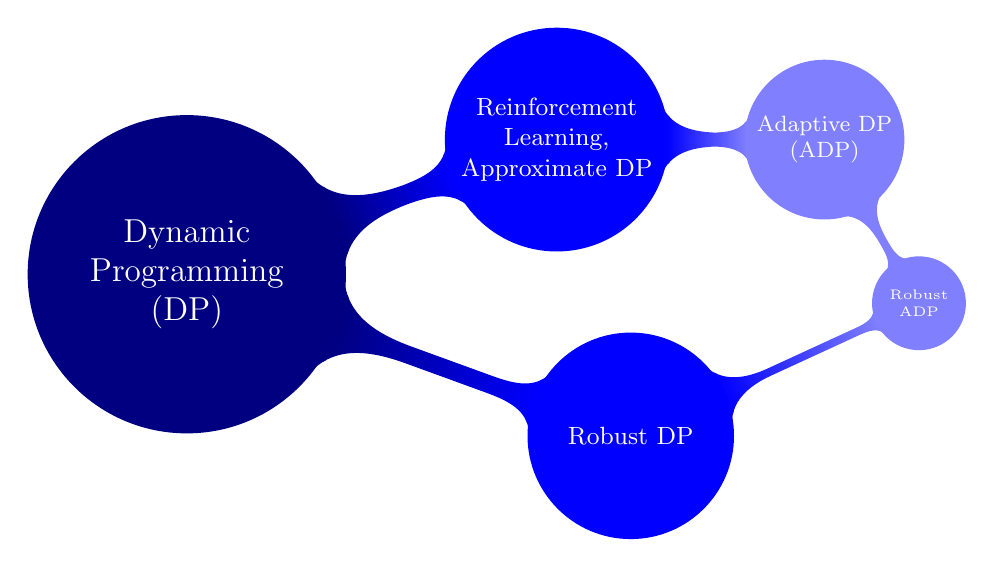
\begin{tikzpicture}[mindmap, concept color=blue!50!black, text=white, level 2/.append style={level distance=3.4cm}]
    \node [concept, text width=2.5cm] at (-9,-16)  {Dynamic Programming (DP)}
    child[concept color=blue, grow=20] {node[concept, text width=2.5cm] {Reinforcement Learning, Approximate DP}
        child[concept color=blue!50,grow=0]{node[concept,  text width=1.8cm] {Adaptive DP\\ (ADP)}
              child[grow=-60]{node[concept] (radp) {Robust ADP}}
%              child[grow=180]{node[concept]{LSTD($\lambda$)}}
%              child[grow=-120]{node[concept]{LSPE($\lambda$)}}
              }
%         child[concept color=blue!50,grow=60]{node[concept]  {LSPI}}
      }
%      child[concept color=blue, grow=40]{node[concept]{Q-learning}[clockwise from=60]
%                  child[concept color=blue!50]{node[concept]{Watkins' Q-learning}}
%                  child[concept color=blue!50,grow=0]{node[concept]{SARSA}}
%                  child[concept color=blue!50,grow=120]{node[concept]{Q-factor API}}
%                  }
%      child[concept color=blue, grow=0]{node[concept]{Actor-critic algorithm}}
%      child [concept color=blue, grow=-40]{ node[concept] {Real-time DP}}
%      child [concept color=blue, grow=-80]{ node[concept] {Linear programming DP} }
%      child[concept color=blue, grow=-120]{node[concept]{Aggregation}}
      child[concept color=blue, grow=-20, level distance=6cm]{node[concept, text width=2.5cm](rdp){Robust DP}};
%  \end{scope}
  \begin{pgfonlayer}{background}
    \draw (rdp) to [circle connection bar switch color=from (blue) to (blue!50)] (radp);
  \end{pgfonlayer}

\end{tikzpicture}
%\end{figure*}

\end{document}